\subsection{Harmonizer}

Harmonizer is structure which detunes input signal slightly to get different "players" play
slightly out of tune as in the real orchestra section. The block diagram of the harmonizer
is shown in figure \ref{fig_harm}

In harmonizer structure there are four channels which are windowed with four sinusoidal windows
that are 90 degrees more out of phase than previous. To decrease the beating effect that is present
in the current chorus there is added some random variance to the detuning of the sound. That means
that each window is slightly differently out of tune. That is as well related to the real world as the players
usually do not play whole music piece in same detuning. \cite{dudas}
\begin{figure}[ht]
\centering
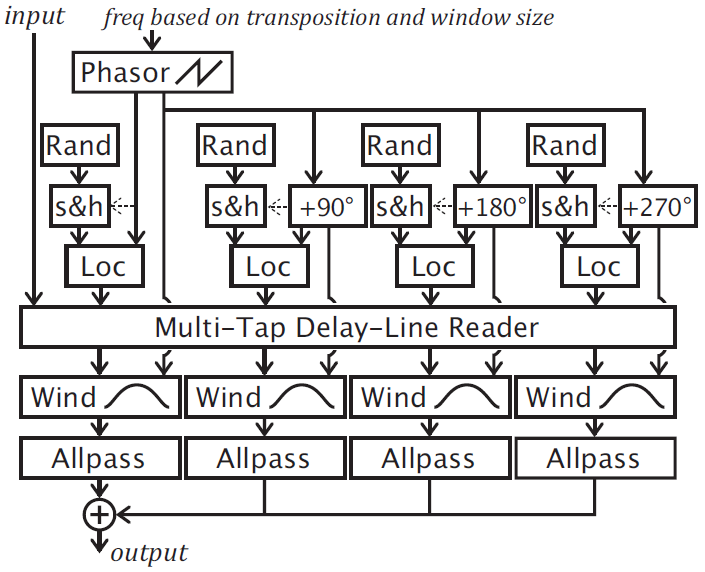
\includegraphics[width = 8cm]{harmonizer.png}
\caption{Chorus Harmonizer Block Diagram. \cite{dudas}}
\label{fig_harm}
\end{figure}

The detuning is made with multi-tap delay-line which is modulated with phasor signal which is basic sawtooth
wave form. After that each channel is windowed by using Hanning window and after that it is allpass filtered.
The windows are triggered with phasor signal and it as well triggers the randomization for each window.
After allpass fitering all the channels are summed together. \cite{dudas}
